\documentclass[prl,twocolumn]{revtex4-2}

\usepackage{graphicx}
\usepackage{color}
\usepackage{latexsym,amsmath}

\definecolor{linkcolor}{rgb}{0,0,0.65} %hyperlink
\usepackage[pdftex,colorlinks=true, pdfstartview=FitV, linkcolor= linkcolor, citecolor= linkcolor, urlcolor= linkcolor, hyperindex=true,hyperfigures=true]{hyperref} %hyperlink%



\begin{document}

\title{Group2601 -- Breast cancer classification via Deep Neural Networks}

\author{Matteo Renato Calcagni}
\author{Nicola Lavarda}
\author{Pasquale Andreacchio}
\author{Agostina Gonzati}

\date{\today}


\begin{abstract}
Breast cancer is one of the most common kind of cancer in our society, carrying a high prevalence among women. For this reason, a regular mammogram screening is recommended every 1--2 years for early detection. 
Once a potential mass is found, it is of key importance to immediately check and classify its nature, that can be either malignant (cancer) or benign (not cancer). Diagnostic misclassifications, particularly false negatives, can lead to life-threatening consequences by delaying critical treatment; therefore, it is of paramount importance to find an algorithm that is able to correctly classify the masses. \\
We thus decided to address this task building a Deep Neural Network (DNN) optimized on binary classification, trained on the Wisconsin diagnostic dataset. Utilizing Optuna for hyperparameter tuning, our model yields a macro F1-score of 0.972 on a held-out test set, with only 1 false negative out of 114 samples. These results underscore the potential of deep learning architectures as highly reliable tools for clinical decision support.
\end{abstract}


\maketitle

\section{Introduction}

Breast cancer remains one of the most frequently diagnosed malignancies and a leading cause of cancer-related mortality among women worldwide. Early detection and accurate classification are the absolute cornerstones of effective treatment, playing a critical role in improving patient prognosis and survival rates. Historically, diagnosing breast cancer has relied heavily on the manual interpretation of medical imagery—such as mammograms, ultrasounds, and histopathological slides—by skilled radiologists and pathologists. While foundational to modern medicine, this traditional diagnostic process is inherently time-intensive, subjective, and susceptible to human error and inter-observer variability.
\par
As the volume and complexity of medical imaging data continue to grow exponentially, there is a pressing need for robust, automated tools to assist healthcare professionals. In recent years, artificial intelligence has emerged as a transformative force in overcoming these diagnostic bottlenecks. Deep learning, has fundamentally revolutionized computer vision and medical image analysis.
\par
Deep Neural Networks (DNNs), in particular, possess the remarkable ability to automatically learn and extract complex, hierarchical features directly from raw data. Unlike traditional machine learning models that require manual feature extraction, DNNs can identify subtle, intricate patterns in cellular structures or breast tissue that might otherwise elude the human eye.
\par
This article explores the application of deep neural networks in breast cancer classification. 
We develop and train a deep neural network able to do this classification task with high confidence. To do so, we use a dataset coming from the state of Wisconsin in the USA, that we obtained from Kaggle \cite{kaggle_breast_cancer} \cite{wolberg1995}. 
\par
We develop the article in 2 chapters: DNN architecture and Results discussion. The first one is meant to accurately describe our network architecture and the method with which we set its hyperparameters, whereas the second one go in deeper details on the network training process and the graphical presentation and analysis of the results. 

\section{DNN architecture}

\subsection{General structure}
The proposed Deep Neural Network (DNN) is a fully connected feedforward neural network, an architecture optimized for binary classification.
To improve training stability, reduce internal covariate shift and accelerate convergence, the network uses \textit{Batch Normalization (BN)} (which normalizes the layer input across the mini-batches, ensuring stable gradient propagation) after each linear transformation in the hidden layers. \par
The architecture is composed of the following sequential components:
\begin{itemize}
    \item \textbf{Input Layer}: Comprises $N$ nodes, where $N$ matches the dimensionality of the standardized feature space extracted from the dataset, in our case \textbf{$N=30$}.
    \item \textbf{Hidden Layers}: The network architecture employs \textbf{three hidden layers}, the first one with 16 neurons, the second one with 8 and the last one with 4. 
    Within each hidden layer, the features go through a linear transformation followed by a \textbf{Batch Normalization} layer.
    \item \textbf{Activation Function}: Following batch normalization, a \textbf{Rectified Linear Unit (ReLU)} activation function is applied to introduce non-linear mapping capabilities to the network.
    \item \textbf{Dropout}: To enhance generalization and mitigate overfitting, a Dropout layer is introduced after the activation function.
    \item \textbf{Output Layer}: Consists of a single neuron with a Sigmoid activation function, mapping the network's final output to a probability score $p \in [0, 1]$. A classification threshold of $0.5$ is subsequently applied to determine the final diagnostic class (0 for benign, 1 for malignant).
\end{itemize}


\subsection{Hyperparameter estimation}
To optimize the performance of our Deep Neural Network, we performed a hyperparameter search using Optuna \cite{optuna}, an automatic and open source hyperparameter optimization framework;
specifically, the tuning process focused on optimizing the \textit{learning rate} and the \textit{dropout rate}, obtaining a learning rate $\eta \approx 0.029$ and a dropout rate $p_\text{drop} = 0.2$. \par
Optuna allowed us to explore the hyperparameter space in a computationally efficient way, identifying the configuration that maximized the evaluation metrics, and thus minimizing the loss, while mitigating the risk of overfitting. 



\section{Results and discussion}

\subsection{Point 1 -- Classification performance}

The model was evaluated on a held-out test set of 114 samples (71 Benign, 43 Malignant).
Table~\ref{tab:metrics} reports precision, recall and F1-score for both classes,
and Figure~\ref{fig:barchart} visualises these metrics as a bar chart.

\begin{table}[!tbh]
\centering
\caption{Classification metrics on the held-out test set (threshold = 0.5).}
\label{tab:metrics}
\begin{tabular}{lcccc}
\hline\hline
Class & Precision & Recall & F1 & Support \\
\hline
Benign (0)    & 0.986 & 0.972 & 0.979 & 71 \\
Malignant (1) & 0.955 & 0.977 & 0.966 & 43 \\
\hline
Macro avg     & 0.970 & 0.974 & 0.972 & 114 \\
\hline\hline
\end{tabular}
\end{table}

\begin{figure}[!tbh]
    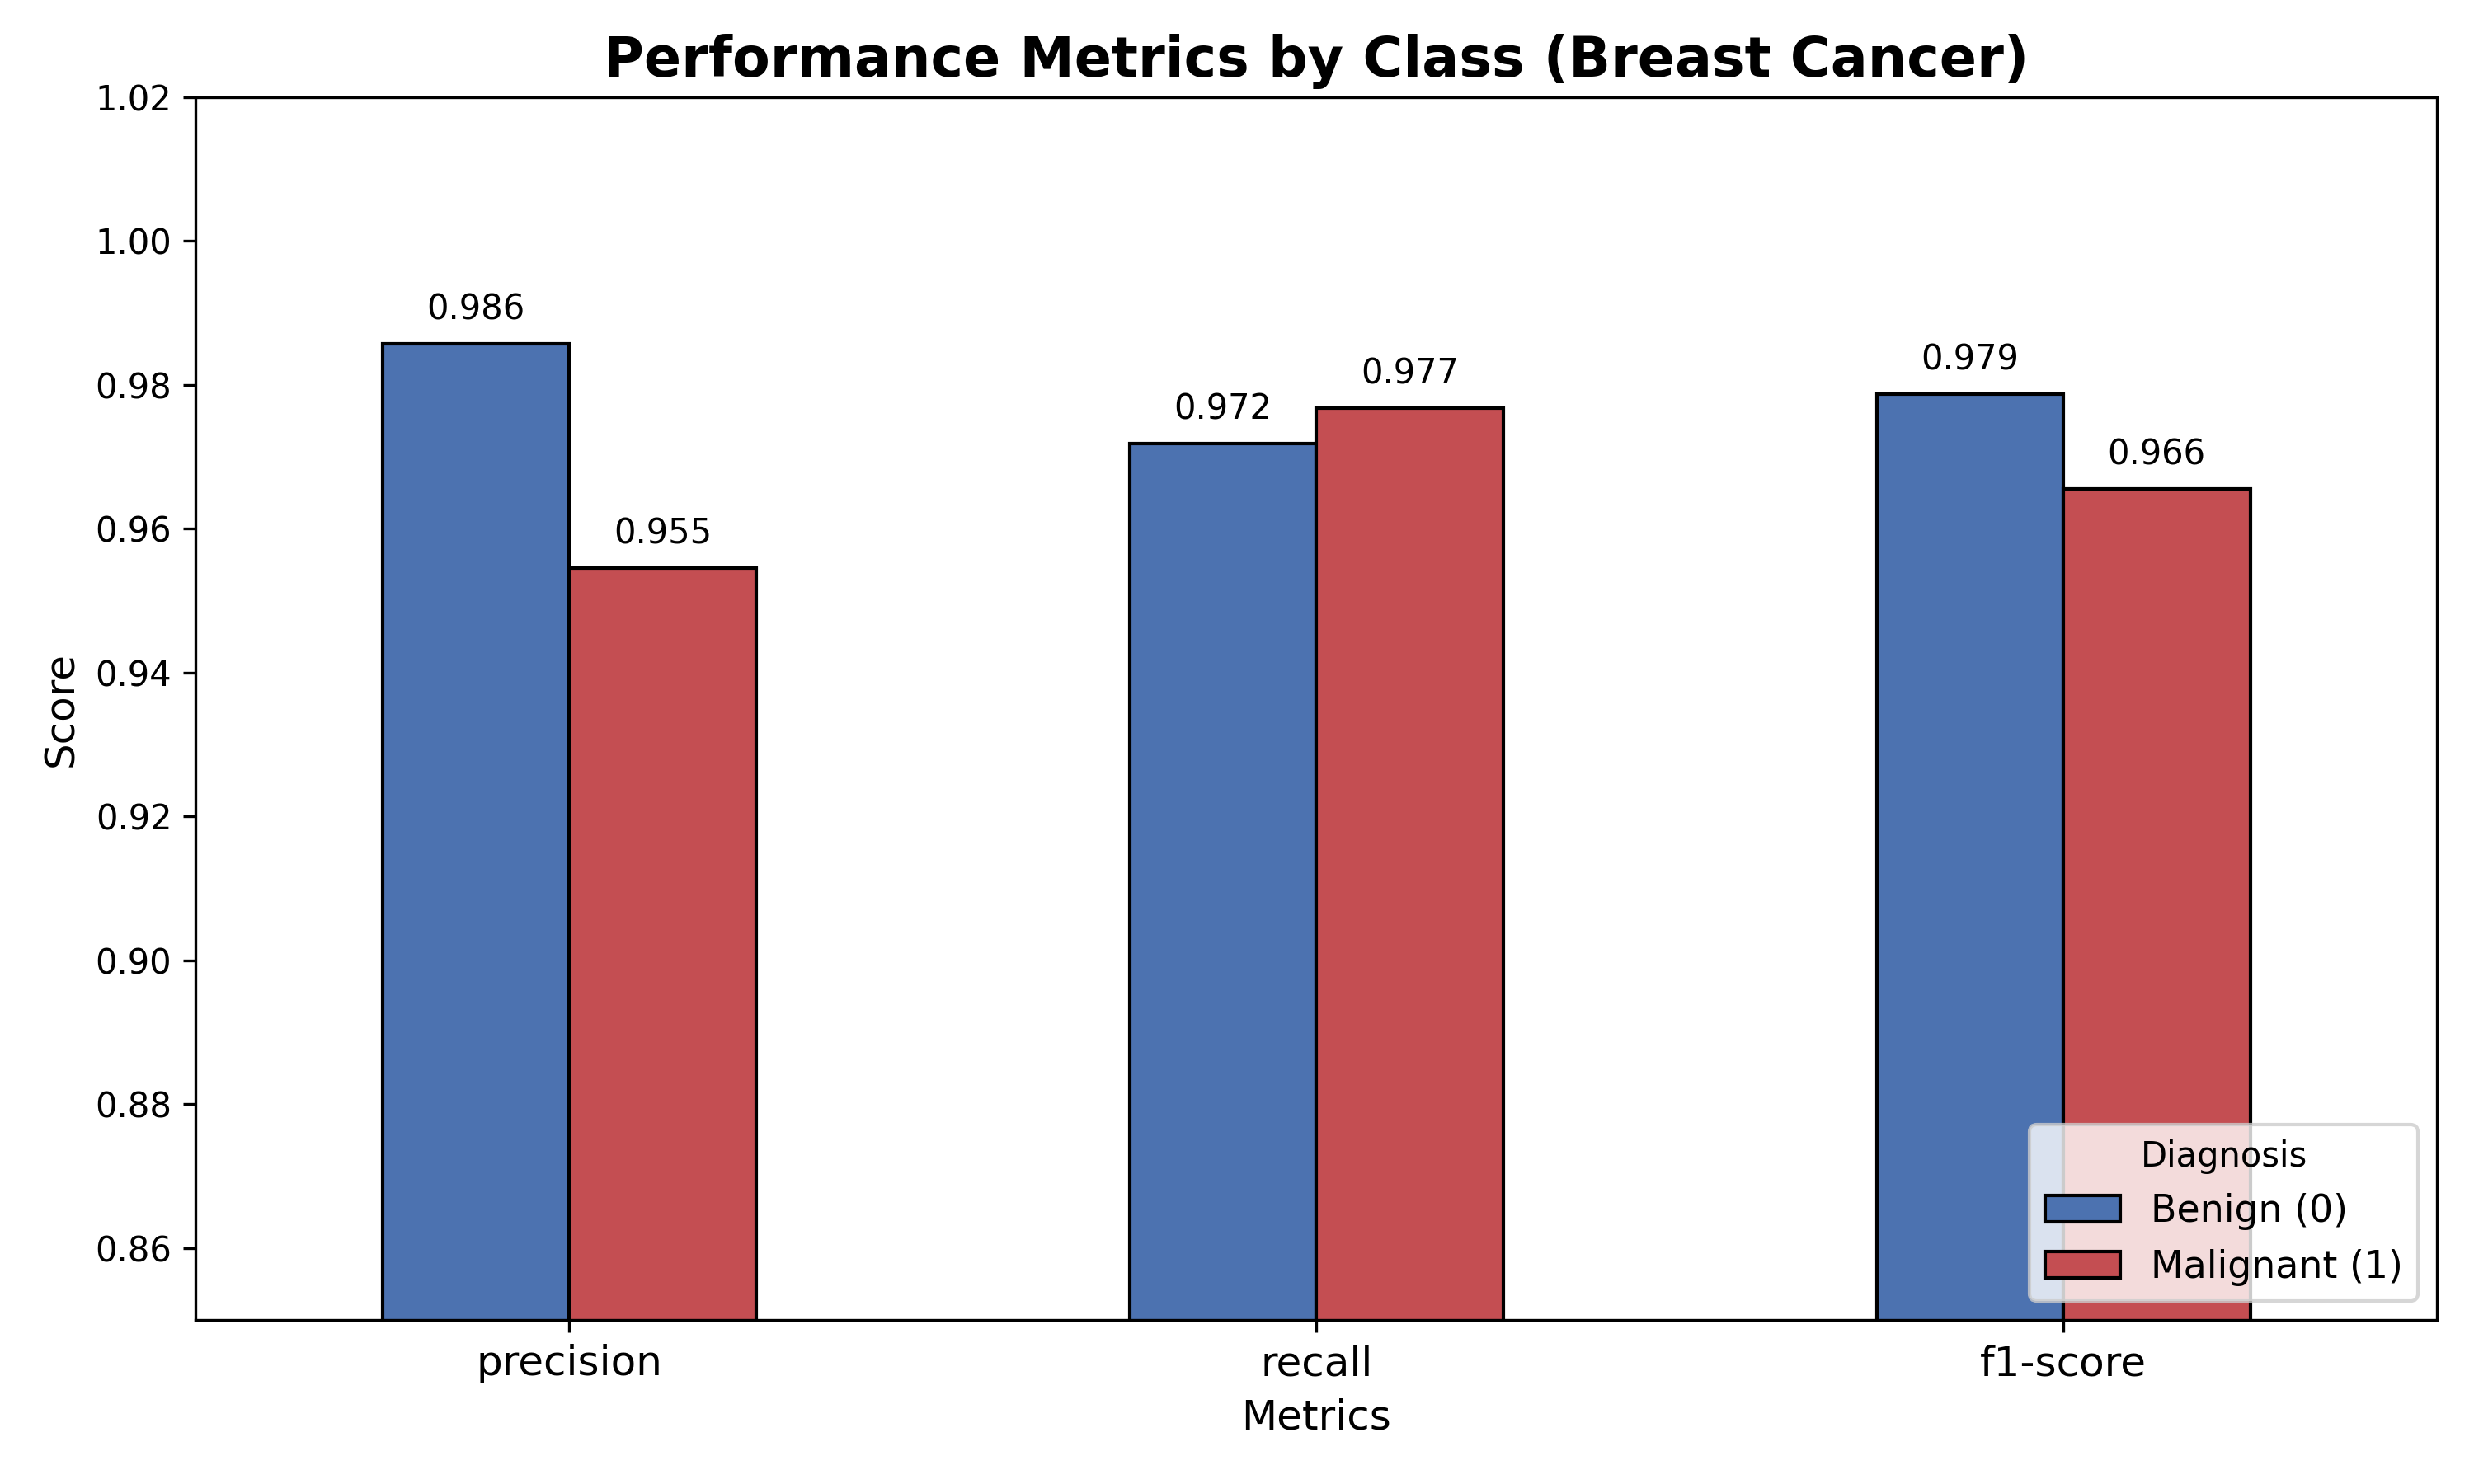
\includegraphics[width=0.44\textwidth]{classification_report_barchart.png}
    \caption{Precision, Recall and F1-score by class (Benign in blue,
             Malignant in red) on the held-out test set.
             All metrics exceed 0.95 for both classes.}
    \label{fig:barchart}
\end{figure}

The confusion matrix is shown in Figure~\ref{fig:cm}. Out of 114 test samples,
only \textbf{3 misclassifications} occur: 2 false positives (benign tumours
incorrectly flagged as malignant) and 1 false negative (a malignant tumour missed
by the model). In a clinical screening context, minimising false negatives is the
absolute priority, as a missed malignancy can have life-threatening consequences.
With only 1 false negative and a recall of 0.977 for the malignant class,
the model provides a clinically strong guarantee for early detection.

\begin{figure}[!tbh]
    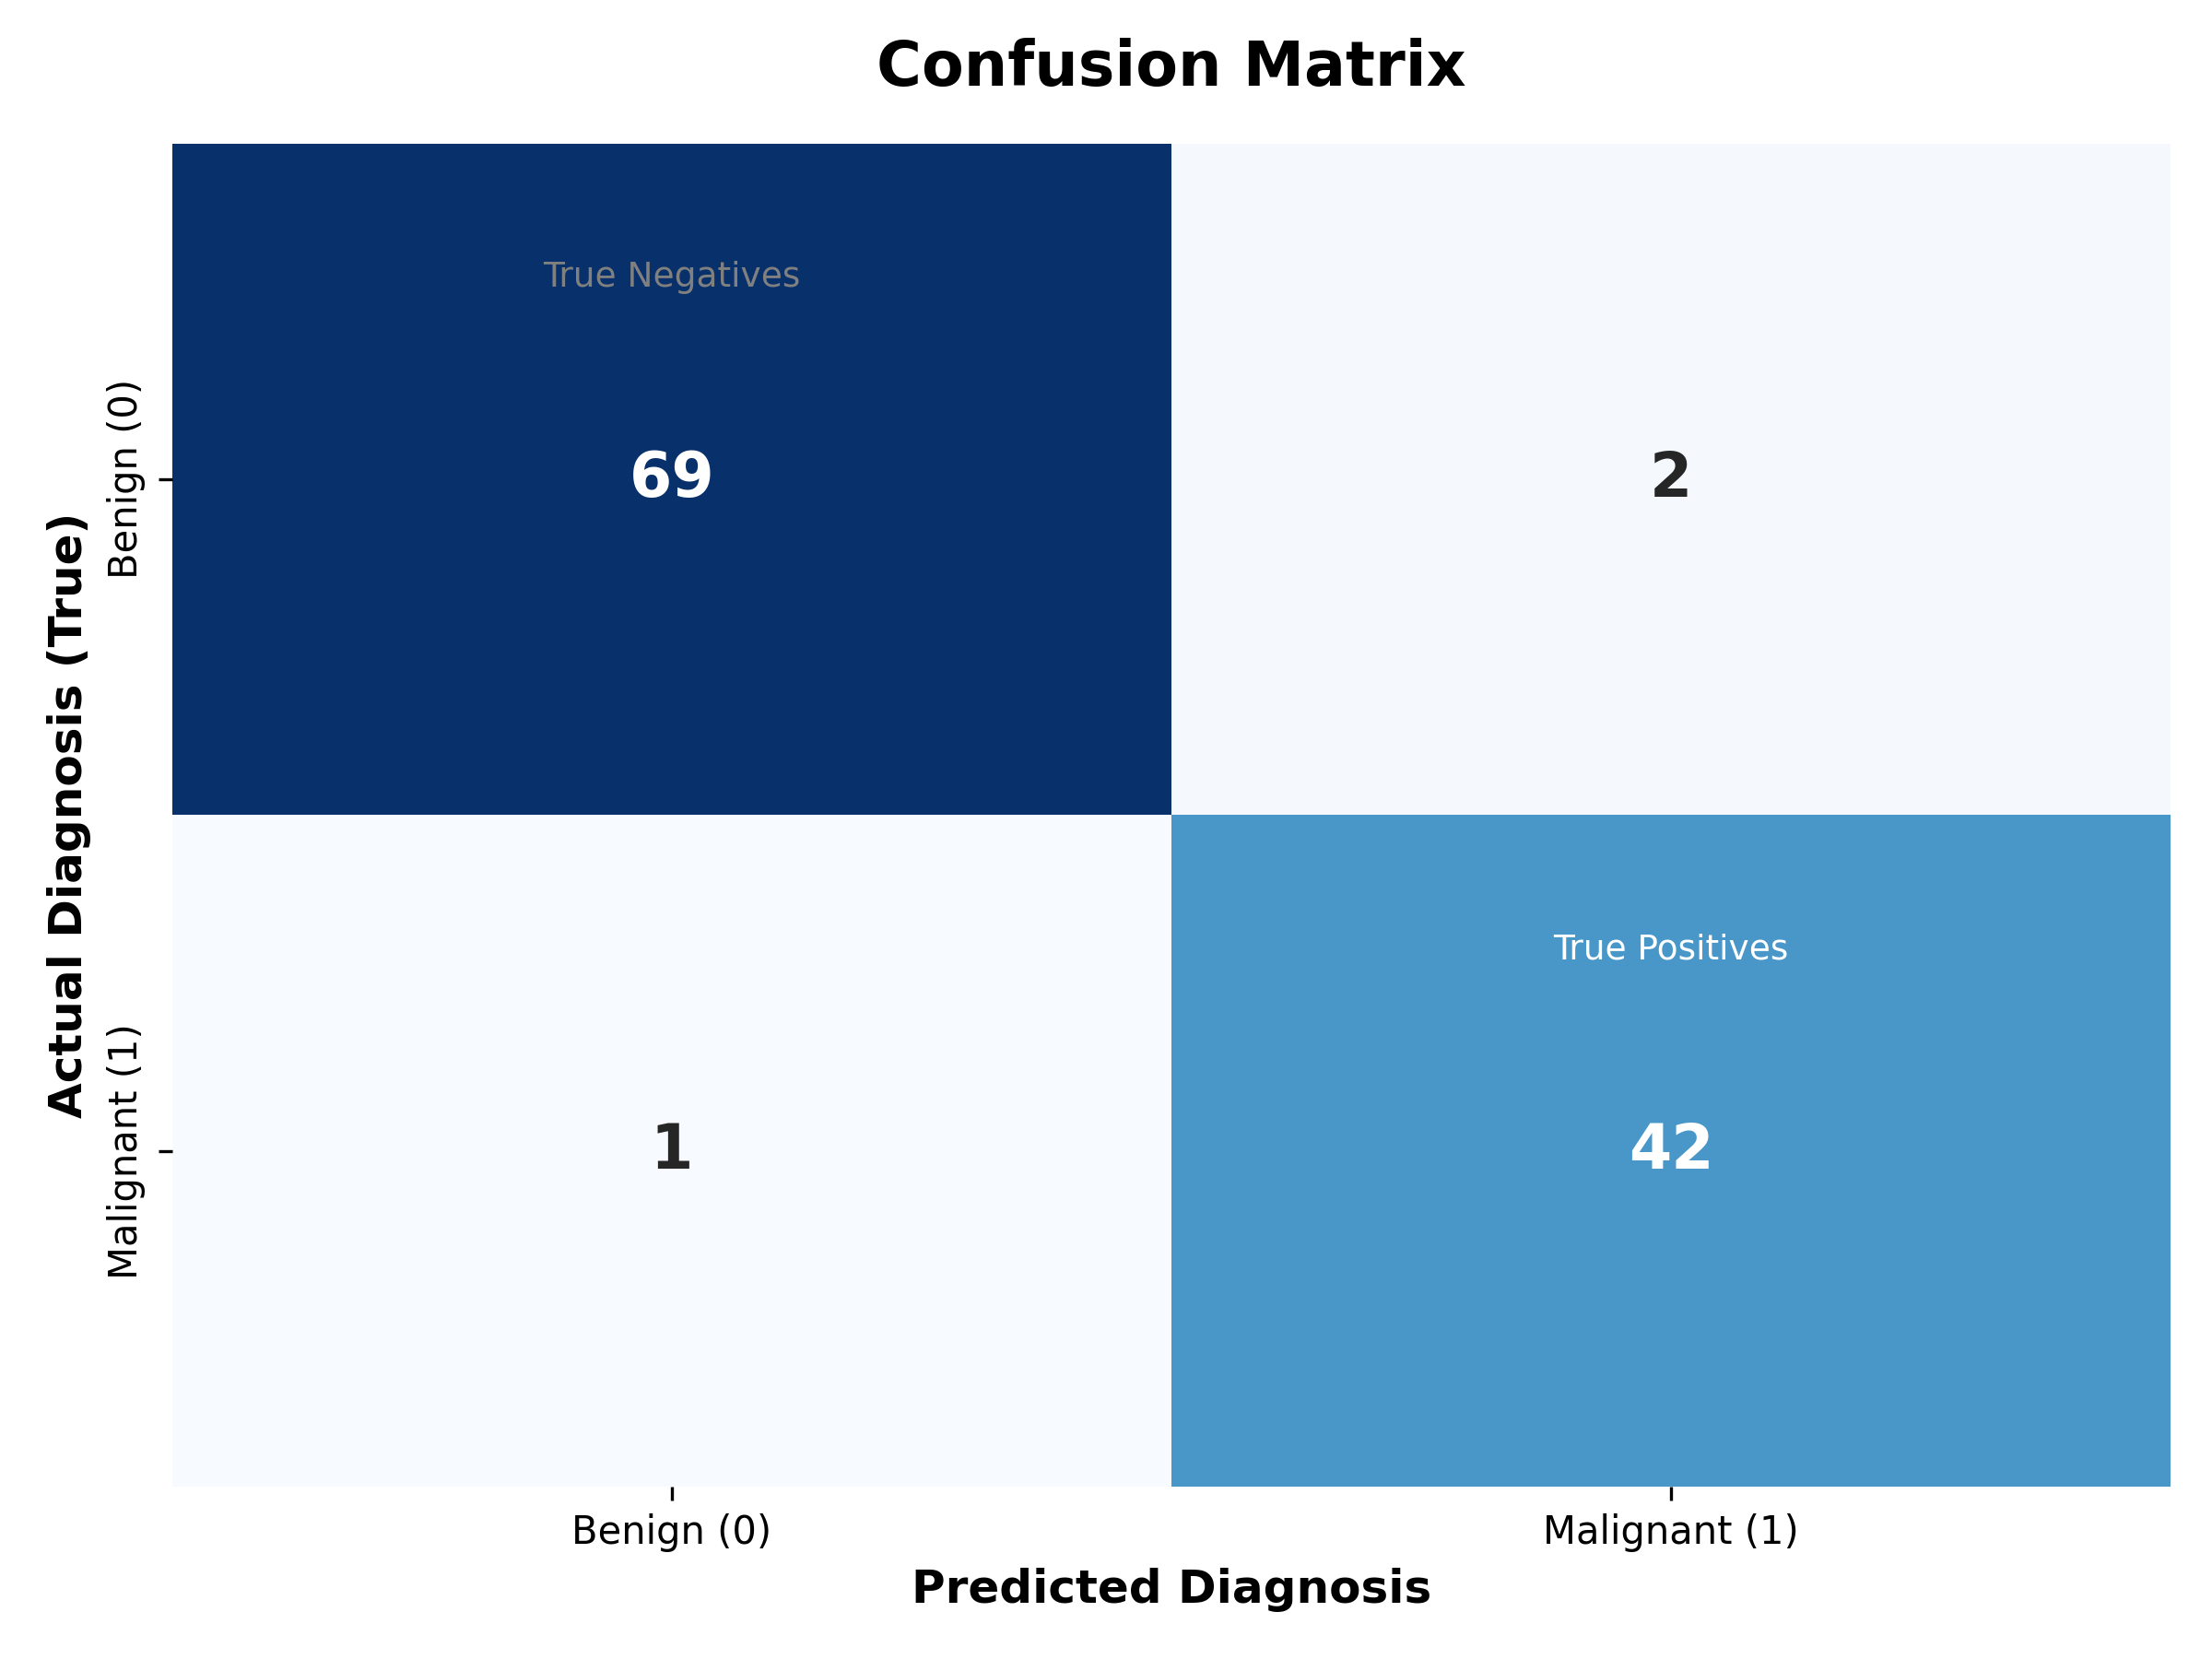
\includegraphics[width=0.44\textwidth]{confusion_matrix.png}
    \caption{Confusion matrix on the held-out test set.
             True Negatives: 69, False Positives: 2,
             False Negatives: 1, True Positives: 42.}
    \label{fig:cm}
\end{figure}

\subsection{Point 2a -- Effect of reducing the training set size}

To study how performance changes with the amount of available training data,
the model was trained on progressively smaller fractions of the training set
(from 5\% to 100\%), using the best hyperparameters found in Point 1.
Each fraction was repeated 3 times with different random seeds and results were averaged.

Figure~\ref{fig:val_loss_both} (left) shows the validation loss as a function of the
number of training samples. The numerical results are summarised in
Table~\ref{tab:reduction}.

\begin{figure}[!tbh]
    \centering
    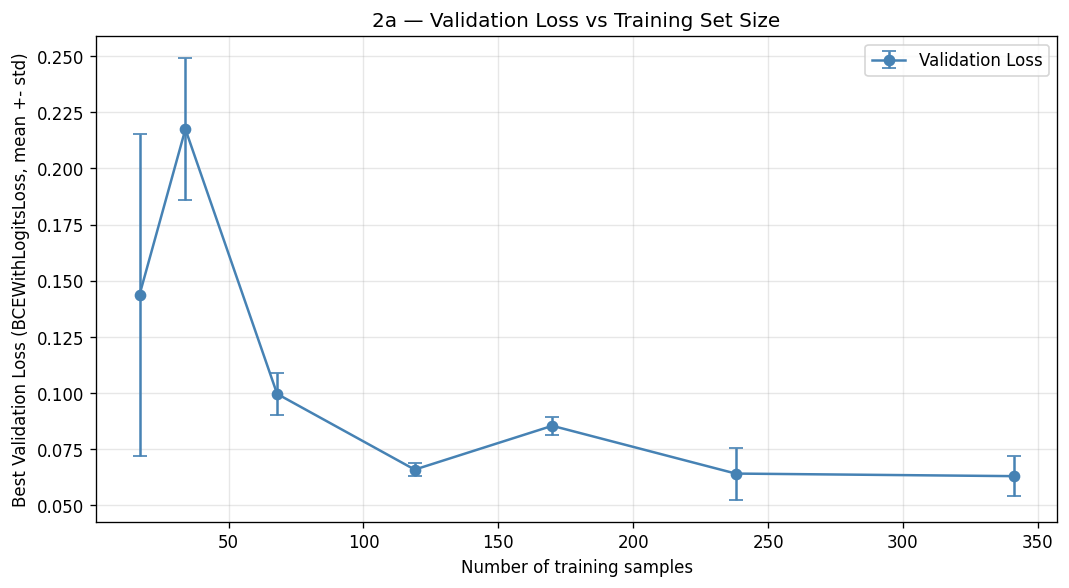
\includegraphics[width=0.23\textwidth]{val_loss_reduction.png}
    \hfill
    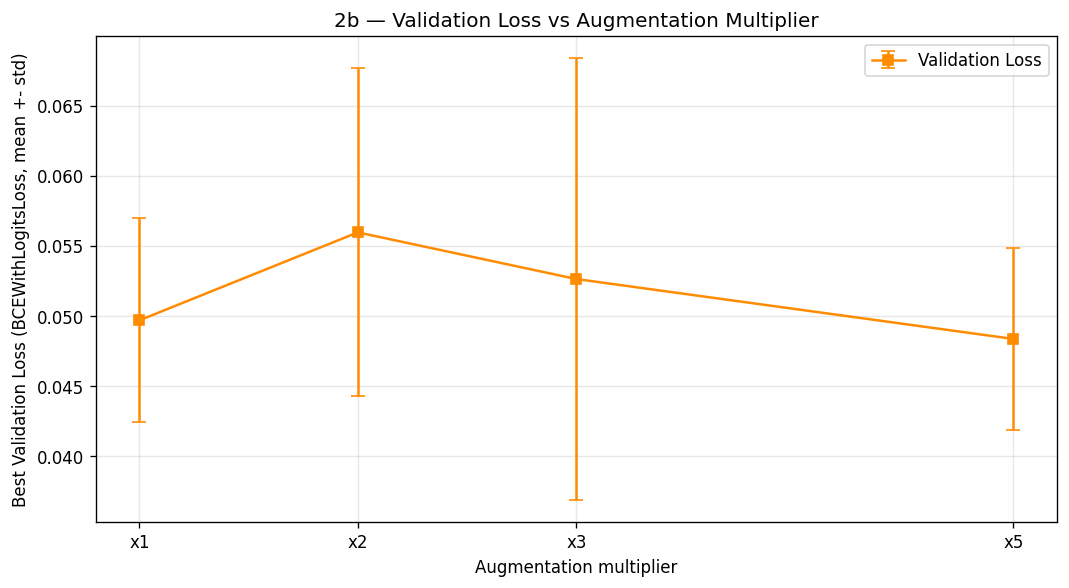
\includegraphics[width=0.23\textwidth]{val_loss_augmentation.png}
    \caption{Best validation loss vs number of training samples (left) and vs augmentation multiplier (right).}
    \label{fig:val_loss_both}
\end{figure}

\begin{table}[!tbh]
\centering
\caption{Data reduction results (mean $\pm$ std over 3 runs).}
\label{tab:reduction}
\begin{tabular}{lccc}
\hline\hline
Fraction & N & F1 macro & Val Loss \\
\hline
5\%   & 17  & $0.937 \pm 0.017$ & $0.144 \pm 0.072$ \\
10\%  & 34  & $0.908 \pm 0.028$ & $0.217 \pm 0.031$ \\
20\%  & 68  & $0.913 \pm 0.028$ & $0.100 \pm 0.009$ \\
35\%  & 119 & $0.959 \pm 0.016$ & $0.066 \pm 0.003$ \\
50\%  & 170 & $0.965 \pm 0.004$ & $0.086 \pm 0.004$ \\
70\%  & 238 & $0.978 \pm 0.004$ & $0.064 \pm 0.012$ \\
100\% & 341 & $0.975 \pm 0.005$ & $0.063 \pm 0.009$ \\
\hline\hline
\end{tabular}
\end{table}

Two key observations emerge. First, even with only 5\% of the training data
(17 samples), the model achieves a macro F1 of 0.937, reflecting the strong
linear separability of the Wisconsin dataset where morphological features carry
substantial discriminative information. Second, the validation loss decreases
monotonically from 0.144 to 0.063 as the training set grows from 5\% to 100\%,
confirming that additional real samples consistently improve generalisation.
The non-monotonic behaviour of the F1 curve at 10--20\% is attributable to
the high variance introduced by small sample sizes in those splits. \par
To further understand the geometrical structure of the data and explain the 
model's remarkable performance with limited training data, we analyzed the 
dataset's global separability. Figure~\ref{fig:pca} shows the 2D PCA 
projection of the standardized feature space. The first principal component 
(PC1) accounts for 44.3\% of the total variance, while the second (PC2) explains 
19.0\%, yielding a cumulative explained variance of 63.3\%. Crucially, the 
projection reveals a clear separation between the benign (blue) and malignant 
(red) classes along the PC1 axis, with the benign samples tightly clustered and 
the malignant ones more dispersed. This high intrinsic linear and non-linear 
separability explains why even a tiny training subset (17 samples) is sufficient 
for the neural network to identify the decision boundary and achieve a high 
macro F1-score of 0.937.

\begin{figure}[!tbh]
    \centering
    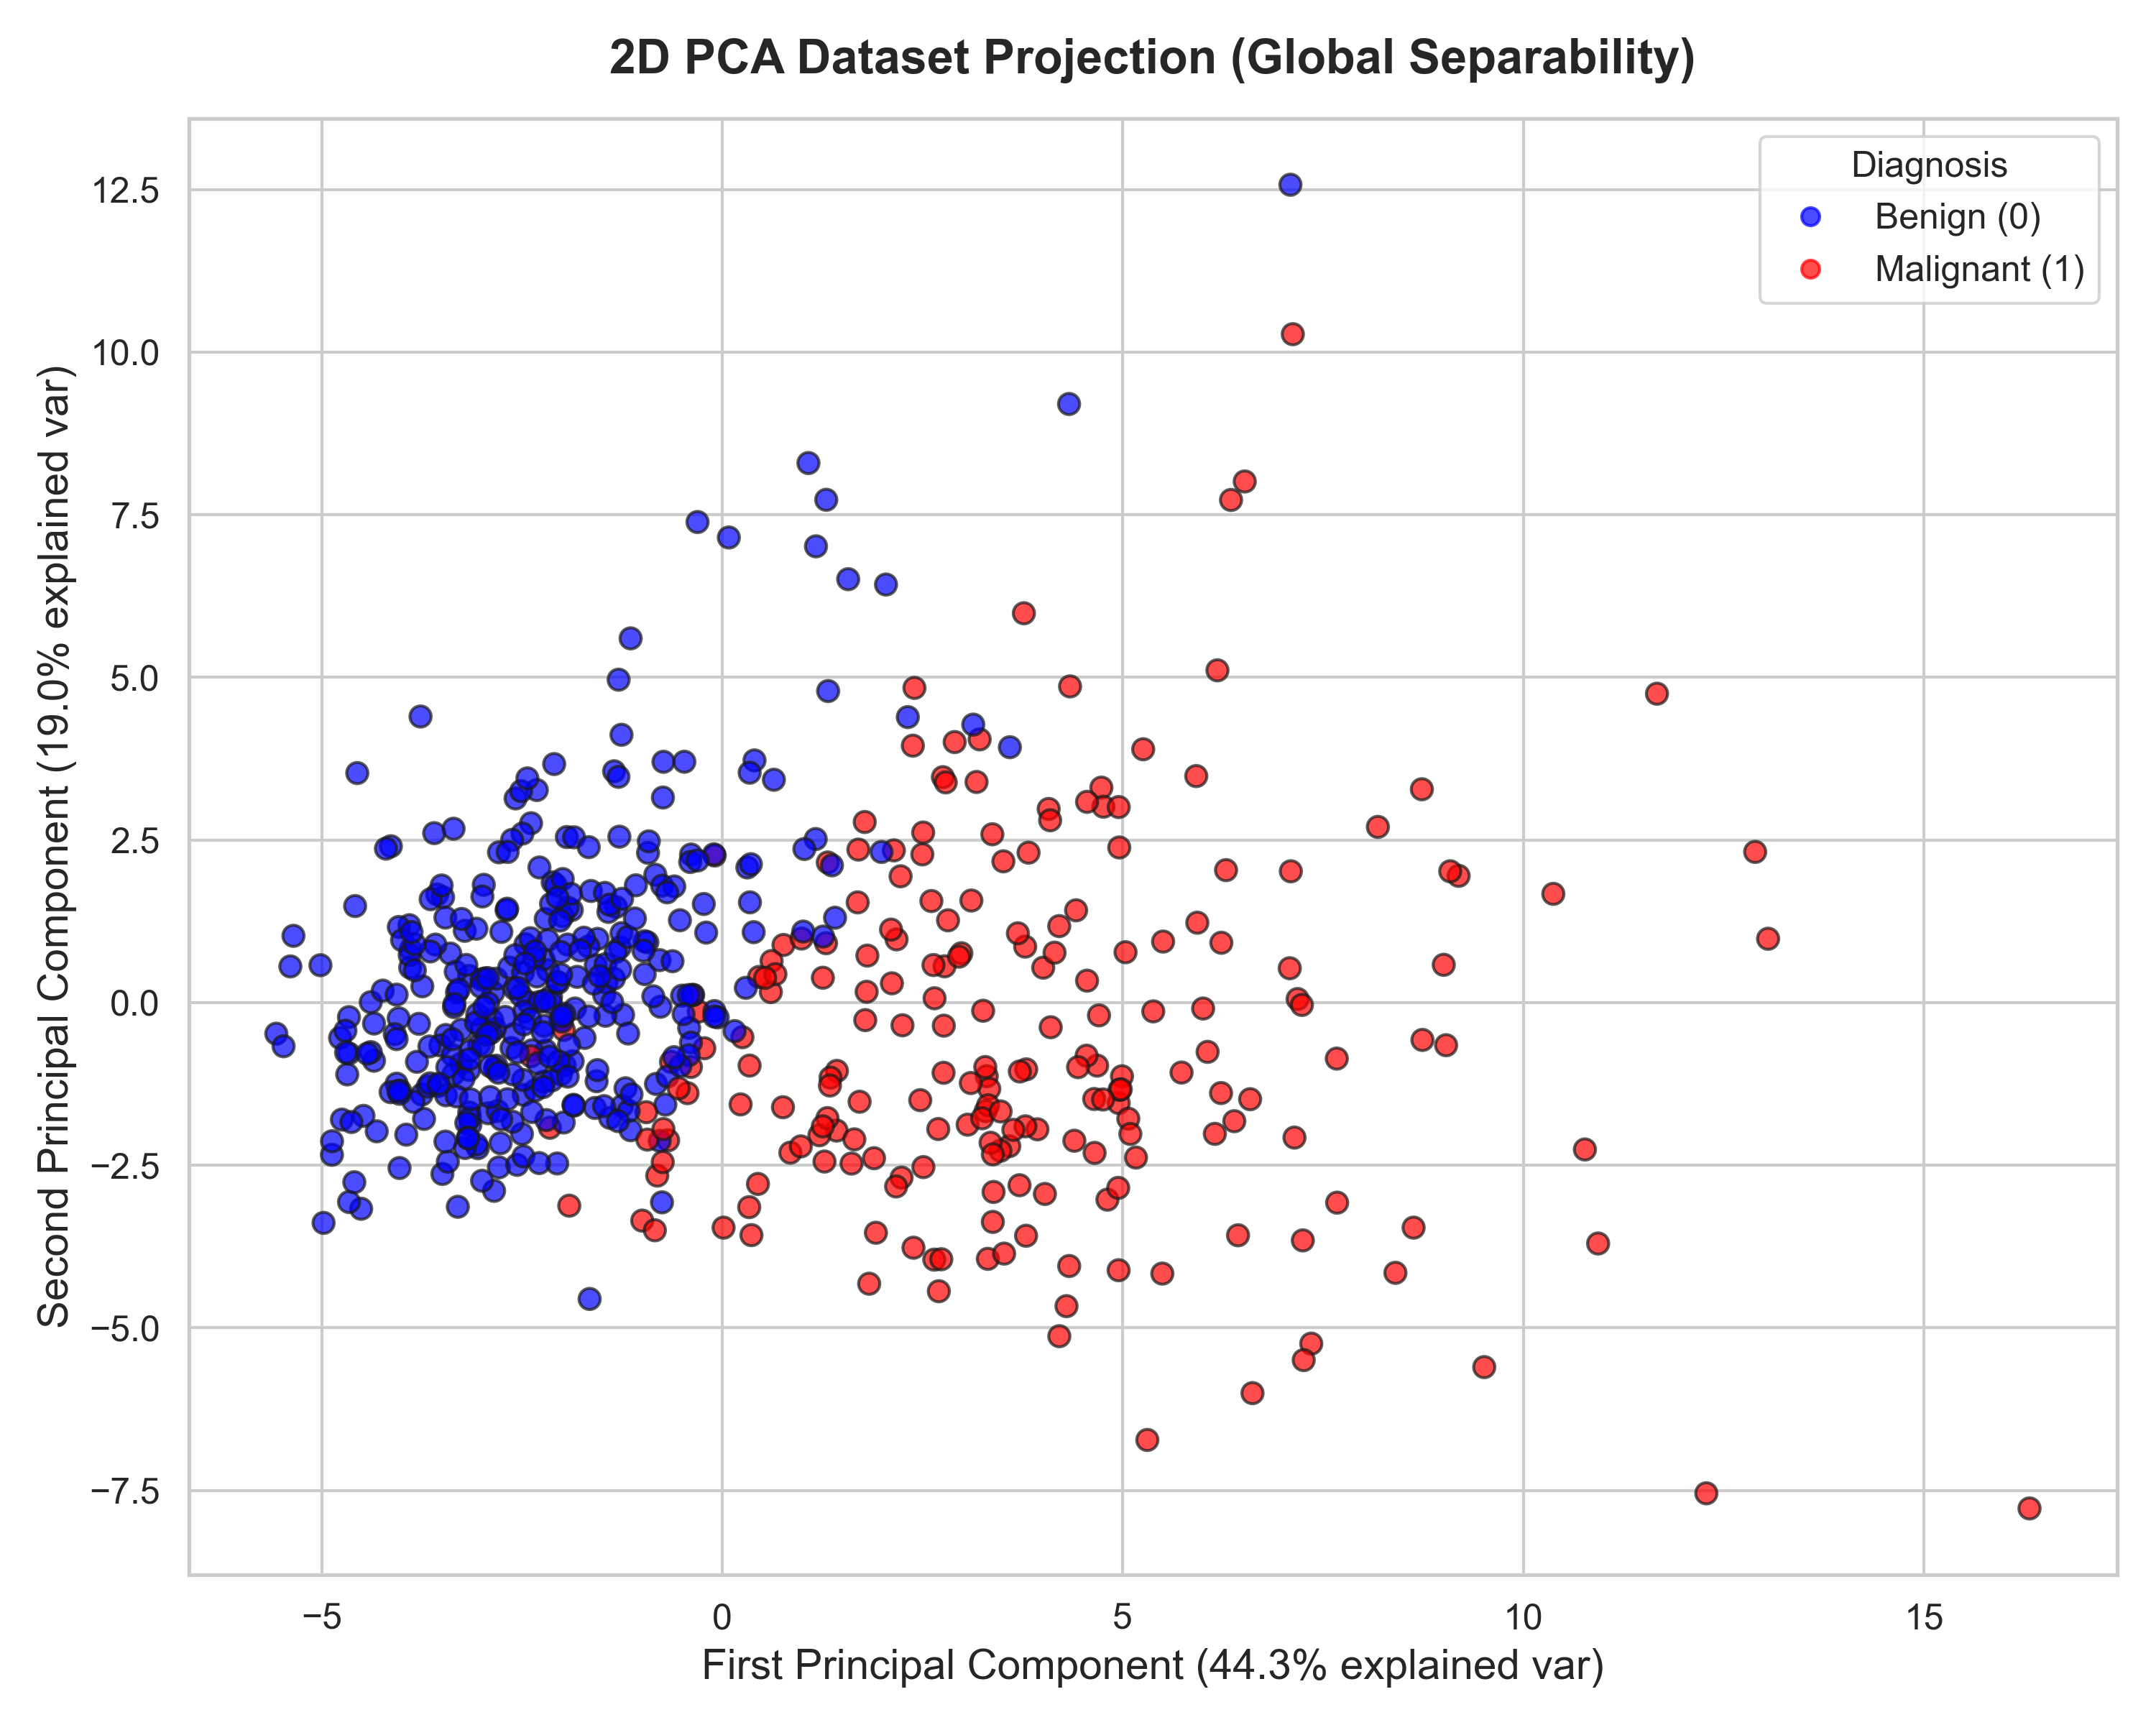
\includegraphics[width=0.44\textwidth]{04_pca_2d_projection.png}
    \caption{2D PCA projection of the standardized dataset. The first principal component (PC1) accounts for 44.3\% of the variance, showing strong class separation between benign (blue) and malignant (red) tumors.}
    \label{fig:pca}
\end{figure}

\subsection{Point 2b -- Effect of Gaussian noise augmentation}

Gaussian noise augmentation ($\sigma = 0.05$ in standardised feature space) was applied
to the training set at multipliers $\times$1 (baseline), $\times$2, $\times$3 and $\times$5.
Both classes were augmented proportionally, preserving the original class ratio.
Table~\ref{tab:augmentation} summarises the numerical results.

\begin{table}[!tbh]
\centering
\caption{Augmentation results (mean $\pm$ std over 3 runs).}
\label{tab:augmentation}
\begin{tabular}{lccc}
\hline\hline
Multiplier & N train & F1 macro & Val Loss \\
\hline
$\times$1 & 341  & $0.978 \pm 0.009$ & $0.050 \pm 0.007$ \\
$\times$2 & 682  & $0.968 \pm 0.012$ & $0.056 \pm 0.012$ \\
$\times$3 & 1023 & $0.963 \pm 0.015$ & $0.053 \pm 0.016$ \\
$\times$5 & 1705 & $0.956 \pm 0.004$ & $0.048 \pm 0.007$ \\
\hline\hline
\end{tabular}
\end{table}

Figure~\ref{fig:val_loss_both} (right) shows the validation loss as a function of the 
augmentation multiplier. The loss remains approximately flat across all 
multipliers (0.048--0.056), indicating that augmentation neither helps nor 
significantly harms generalisation.

The baseline ($\times$1, F1 = 0.978) is the best-performing configuration.
F1 decreases slightly but consistently as the augmentation multiplier increases,
reaching 0.956 at $\times$5, while the validation loss remains essentially flat.
This indicates that the model has already learned the data manifold from the
original samples: adding Gaussian perturbations introduces noise without providing
new discriminative signal. Figure~\ref{fig:f1_both} shows the macro F1-score for both Point 2a (left) and Point 2b (right).

\begin{figure}[!tbh]
    \centering
    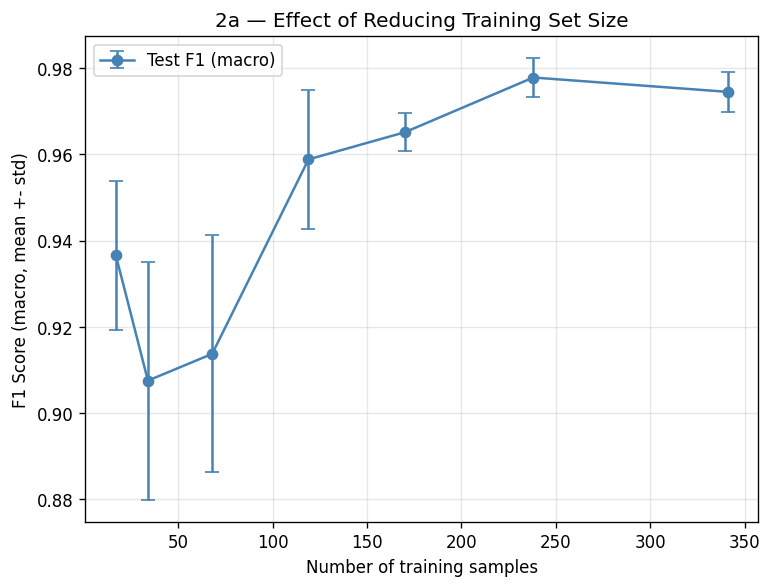
\includegraphics[width=0.23\textwidth]{augmentation_f1_a.png}
    \hfill
    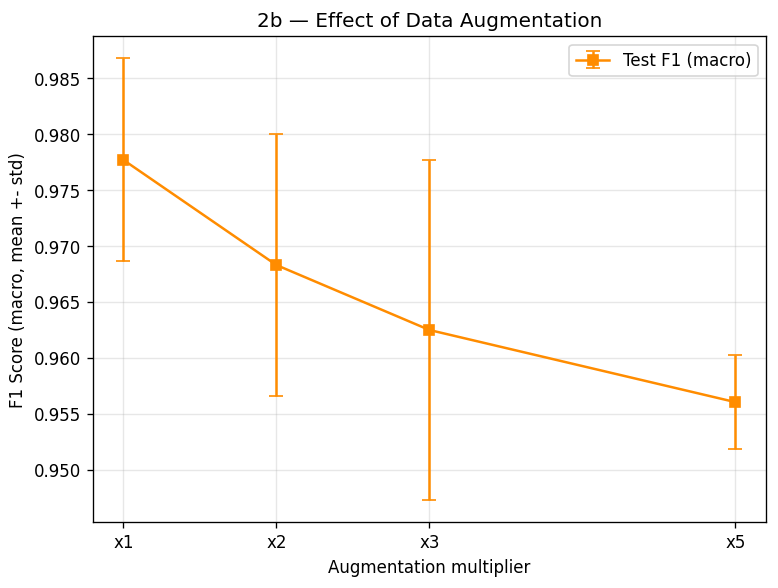
\includegraphics[width=0.23\textwidth]{augmentation_f1_b.png}
    \caption{Macro F1-score vs number of training samples (left) and vs augmentation multiplier (right). Error bars represent $\pm$ standard deviation over 3 runs.}
    \label{fig:f1_both}
\end{figure}


Finally, Figure~\ref{fig:comparison} directly compares performance achieved 
by reducing real data (Point 2a) against augmenting with synthetic data 
(Point 2b) at equivalent total sample counts. Real samples consistently 
outperform synthetic ones, confirming that Gaussian noise augmentation 
cannot replicate the discriminative value of genuine observations on a 
dataset where features already carry strong biological signal.

\begin{figure}[!tbh]
    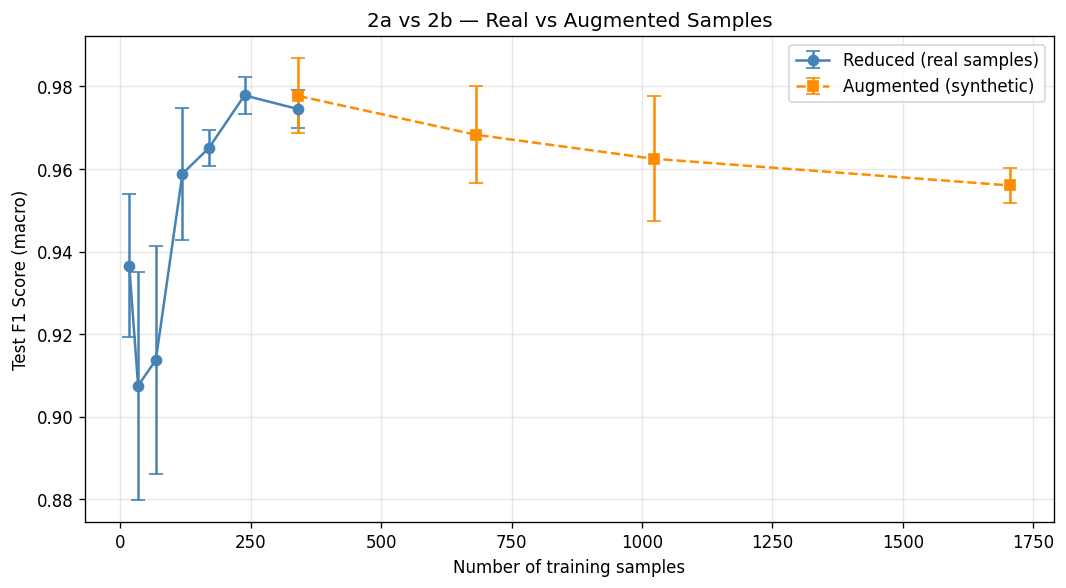
\includegraphics[width=0.44\textwidth]{real_vs_augmented.png}
    \caption{Test macro F1-score vs number of training samples:
             real data reduction (blue solid) vs Gaussian noise
             augmentation (orange dashed). Real samples consistently
             outperform synthetic ones at equivalent counts.}
    \label{fig:comparison}
\end{figure}

\subsection{Point 3 -- Interpretability and Feature Importance via SHAP}

To transition from global data geometry to model interpretability, we performed a SHAP (SHapley Additive exPlanations) analysis on the test predictions. This approach allows us to inspect both global feature importance and the local decision-making process. Figure~\ref{fig:shap_analysis} (left) displays the SHAP summary beeswarm plot, ranking features by their mean absolute SHAP values. The most influential feature is \texttt{concave points\_mean}, followed by \texttt{texture\_worst} and \texttt{radius\_worst}. For these features, high values (represented in red) correspond to positive SHAP values, which push the model output toward malignancy ($y=1$). Biologically, these findings are highly consistent with oncology, where increased nuclear contour irregularities (\texttt{concave points\_mean}) and larger cell sizes (\texttt{radius\_worst}) are key indicators of tumor invasiveness.
Conversely, we observe interesting interaction effects: for instance, features like \texttt{compactness\_mean} exhibit an inverse trend, where lower values contribute positively to malignancy, likely due to collinearity with primary size features in the fully connected network.

To investigate how the model integrates these features for individual diagnoses, we analyze three benchmark cases in Figure~\ref{fig:shap_analysis} (right). Starting from the log-odds base value of $\approx -1.25$ (the expected output before feature contribution), the decision plot traces the cumulative impact of each feature:
\begin{itemize}
    \item \textbf{Benign Case}: Key features like low \texttt{texture\_worst}, low \texttt{radius\_worst}, and low \texttt{concave points\_mean} progressively drive the log-odds output to the left (negative values, ending at $\approx -7.0$), corresponding to a near-zero probability of malignancy.
    \item \textbf{Malignant Case}: High values of these same features push the prediction to the right, ending at a high positive log-odds value ($\approx 7.5$), resulting in high confidence of malignancy.
    \item \textbf{Borderline Case}: The features exert opposing forces, resulting in an intermediate trajectory that terminates around a moderate log-odds score ($\approx -3.5$), highlighting cases that lie closer to the decision boundary.
\end{itemize}
These visualizations provide clinicians with a transparent, step-by-step audit trail for each diagnosis, addressing the traditional 'black-box' limitation of deep learning models in healthcare.

\begin{figure*}[!tbh]
    \centering
    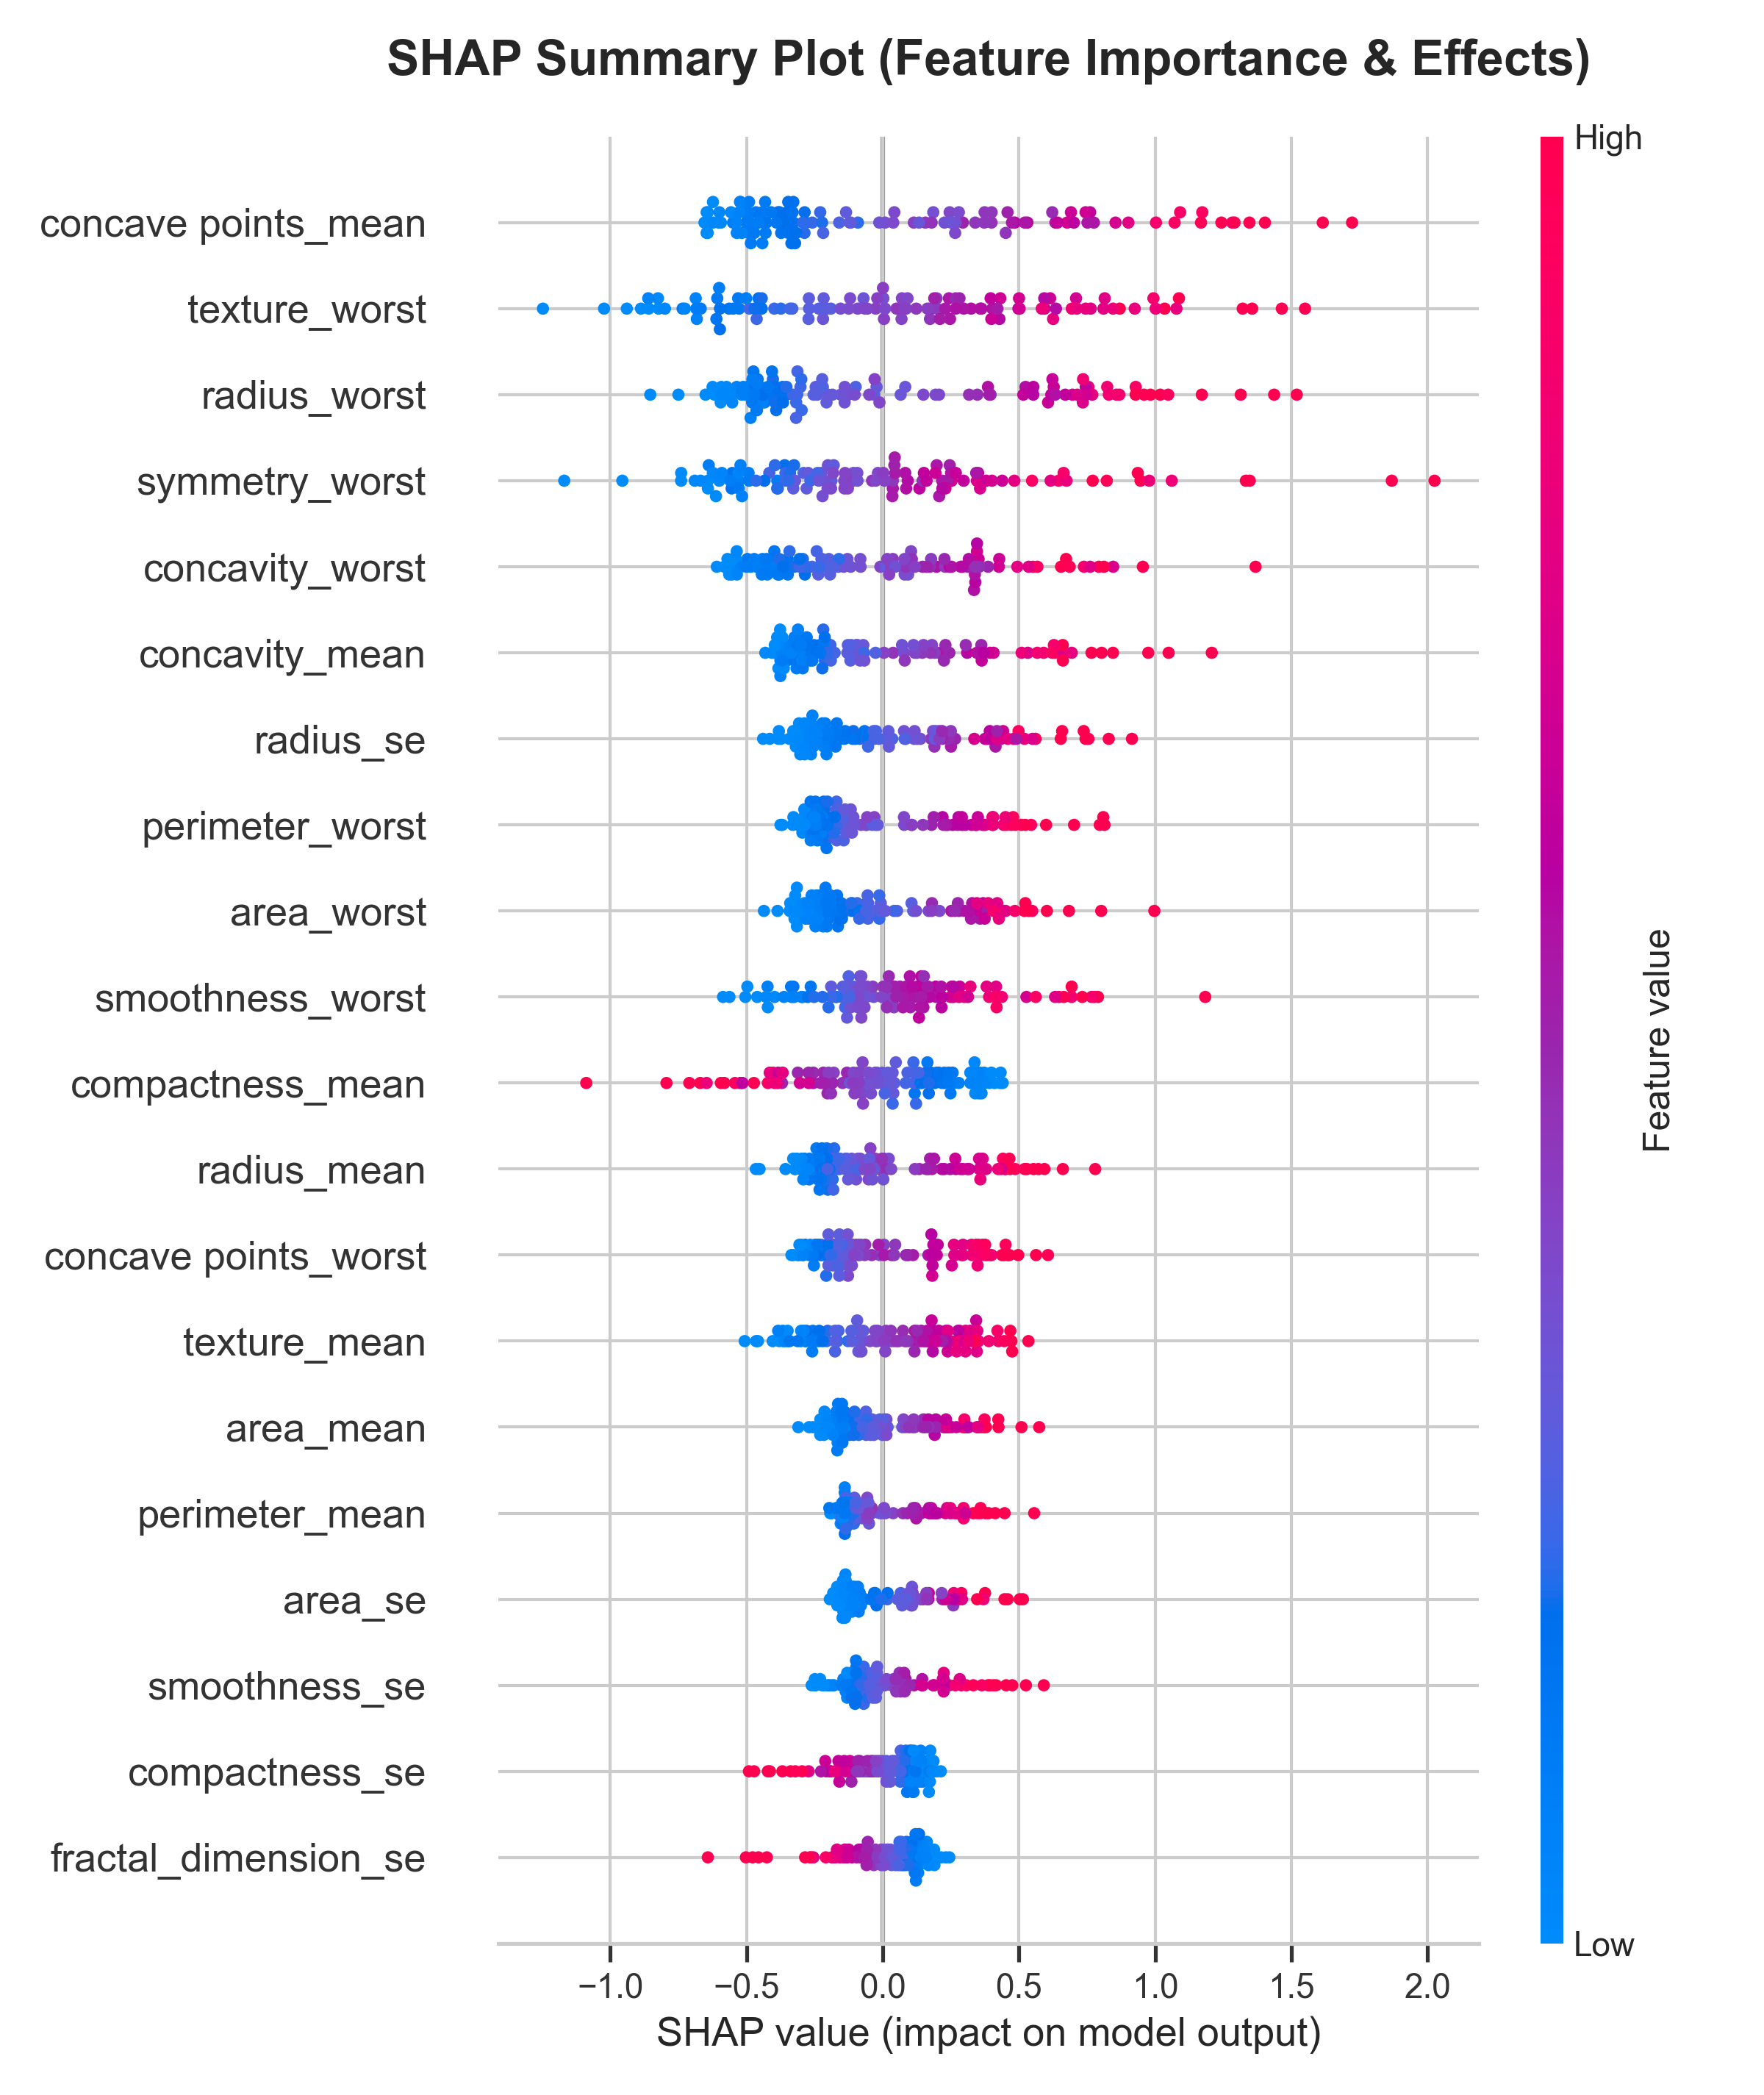
\includegraphics[width=0.4\textwidth]{11_shap_summary_beeswarm.png}
    \hfill
    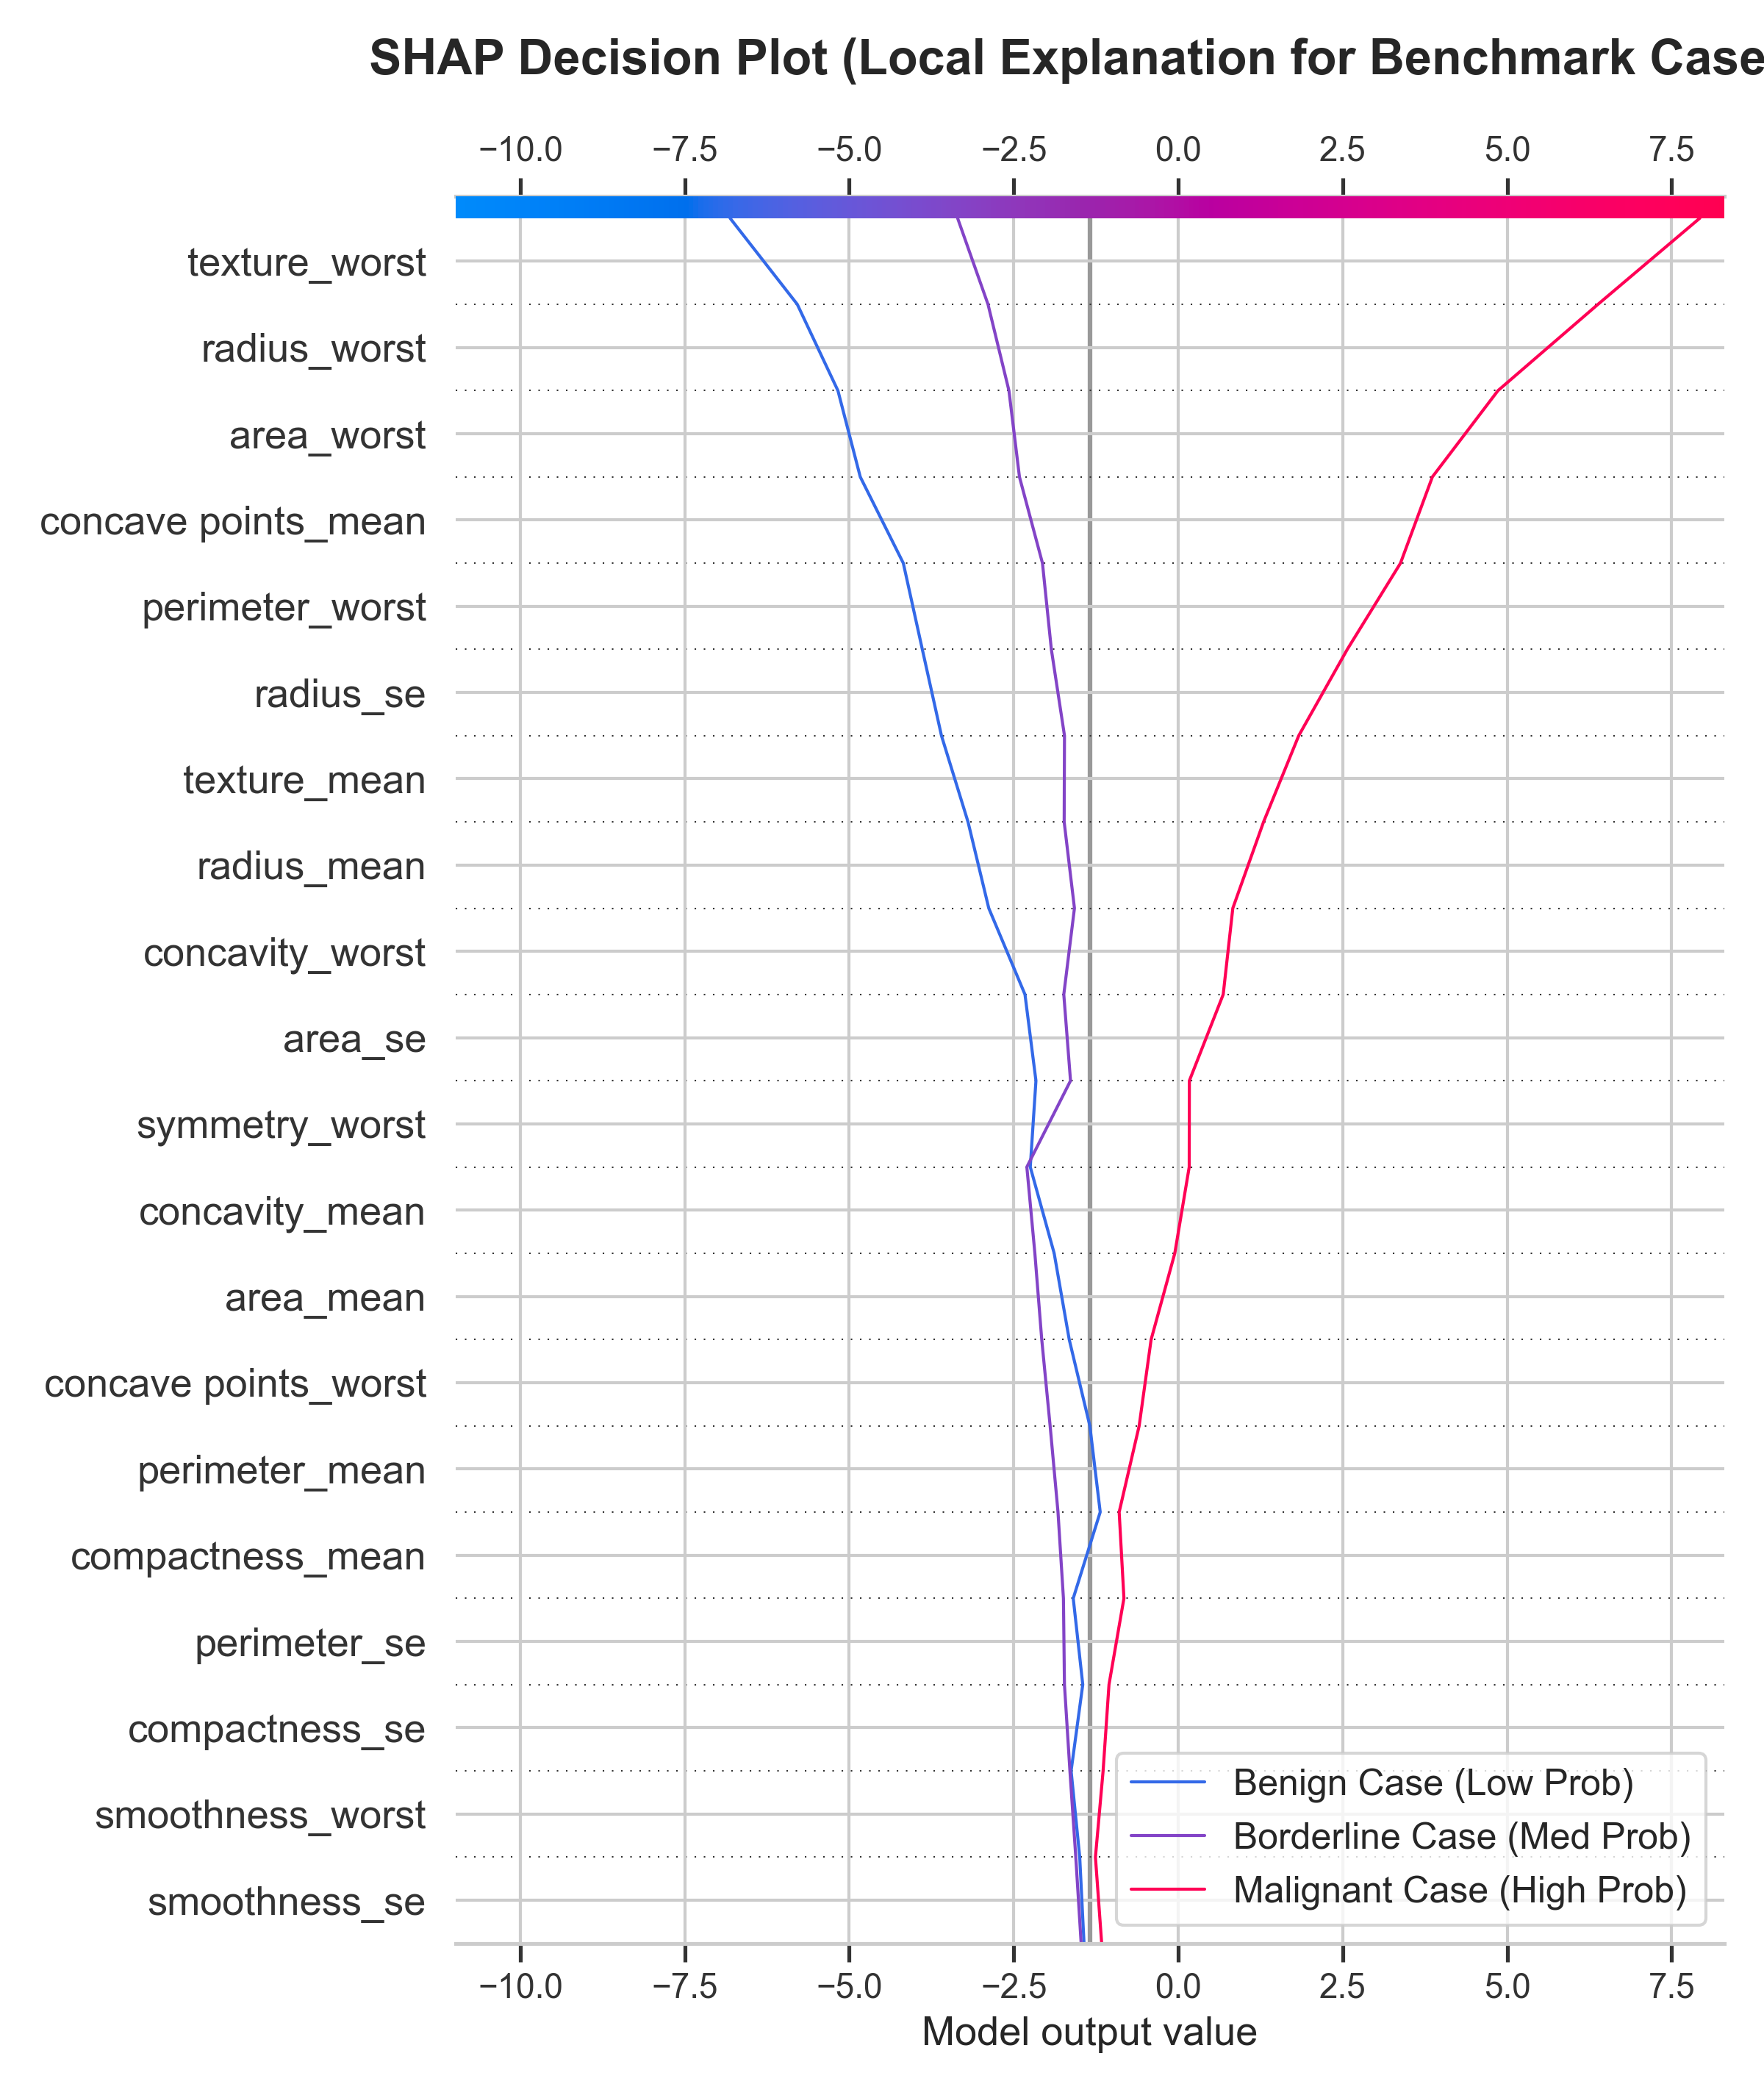
\includegraphics[width=0.4\textwidth]{14_shap_decision_plot_benchmarks.png}
    \caption{Interpretability analysis. Left: SHAP beeswarm summary plot showing global feature importance and the direction of feature effects on model output. Right: SHAP decision plot illustrating the cumulative feature contributions from the base value to the final output for benign, borderline, and malignant benchmark cases.}
    \label{fig:shap_analysis}
\end{figure*}

\section{Conclusions}

We developed and evaluated a fully connected deep neural network for binary
classification of breast tumours (Benign / Malignant) using the Wisconsin
Breast Cancer Dataset~\cite{kaggle_breast_cancer,wolberg1995}.
The main findings are the following.

The hyperparameter search via Optuna identified dropout = 0.2 and lr = 0.0281
as the optimal configuration. The best model achieves a macro F1-score of
0.972, with only 3 misclassifications out of 114 test samples --
critically, only 1 false negative (missed malignancy). With a recall of 0.977
for the malignant class, the network provides a strong guarantee for early
cancer detection.

Regarding data availability, the model maintains high performance even with
very limited training data (F1 = 0.937 at 5\% of samples), reflecting the
strong separability of the morphological features in this dataset.
Additional real samples improve generalisation monotonically, as confirmed
by the decreasing validation loss curve.

Gaussian noise augmentation provides no measurable benefit on this dataset:
F1 slightly decreases at higher multipliers and the validation loss remains flat.
This is consistent with the fact that the dataset already carries rich biological
signal, augmentation is most useful when real data is scarce or poorly structured,
neither of which applies here.


Overall, these results demonstrate that deep neural networks are a highly effective
tool for breast cancer classification, offering near-clinical-grade performance
with a simple architecture when the input features are well-chosen and the
dataset is of sufficient quality.

\begin{thebibliography}{99}

% --- Kaggle breast cancer dataset ---
\bibitem{kaggle_breast_cancer}
  utkarshx27, Kaggle Repository, \url{https://www.kaggle.com/datasets/utkarshx27/breast-cancer-wisconsin-diagnostic-dataset} (2023).

% --- Original UCI Dataset Citation ---
\bibitem{wolberg1995}
  W. H. Wolberg, W. N. Street, O. L. Mangasarian,
  UCI Machine Learning Repository, DOI: 10.24432/C5DW2B (1995).

% --- Optuna Paper ---
\bibitem{optuna}
T. Akiba, S. Sano, T. Yanase, T. Ohta, and M. Koyama, 
``Optuna: A Next-generation Hyperparameter Optimization Framework,'' 
\textit{Proceedings of the 25th ACM SIGKDD International Conference on Knowledge Discovery \& Data Mining}, pp. 2623--2631 (2019).  

\end{thebibliography}



\end{document}
